\documentclass[
11pt, % The default document font size, options: 10pt, 11pt, 12pt
%codirector, % Uncomment to add a codirector to the title page
]{Clases/charter} 


\usepackage{eurosym}

% El títulos de la memoria, se usa en la carátula y se puede usar el cualquier lugar del documento con el comando \ttitle
\titulo{Aplicaciones de modelos de lenguaje de Inteligencia Artificial (LLM) en la ambientación narrativa} 

% Nombre del posgrado, se usa en la carátula y se puede usar el cualquier lugar del documento con el comando \degreename
%\posgrado{Carrera de Especialización en Sistemas Embebidos} 
%\posgrado{Carrera de Especialización en Internet de las Cosas} 
\posgrado{Carrera de Especialización en Inteligencia Artificial}
%\posgrado{Maestría en Sistemas Embebidos} 
%\posgrado{Maestría en Internet de las cosas}

% Tu nombre, se puede usar el cualquier lugar del documento con el comando \authorname
\autor{Ing. Mario Gómez Alonso} 

% El nombre del director y co-director, se puede usar el cualquier lugar del documento con el comando \supname y \cosupname y \pertesupname y \pertecosupname
\director{Por ser definido}
\pertenenciaDirector{Por ser definida} 
% FIXME:NO IMPLEMENTADO EL CODIRECTOR ni su pertenencia
\codirector{John Doe} % para que aparezca en la portada se debe descomentar la opción codirector en el documentclass
\pertenenciaCoDirector{FIUBA}

% Nombre del cliente, quien va a aprobar los resultados del proyecto, se puede usar con el comando \clientename y \empclientename
\cliente{Ing. Hans Manuel Grenner Noguerón}
\empresaCliente{Critical Match}

% Nombre y pertenencia de los jurados, se pueden usar el cualquier lugar del documento con el comando \jurunoname, \jurdosname y \jurtresname y \perteunoname, \pertedosname y \pertetresname.
\juradoUno{Nombre y Apellido (1)}
\pertenenciaJurUno{pertenencia (1)} 
\juradoDos{Nombre y Apellido (2)}
\pertenenciaJurDos{pertenencia (2)}
\juradoTres{Nombre y Apellido (3)}
\pertenenciaJurTres{pertenencia (3)}
 
\fechaINICIO{17 de octubre de 2023}		%Fecha de inicio de la cursada de GdP \fechaInicioName
\fechaFINALPlan{5 de diciembre de 2023} 	%Fecha de final de cursada de GdP
\fechaFINALTrabajo{Por ser definido}	%Fecha de defensa pública del trabajo final


\begin{document}

\maketitle
\thispagestyle{empty}
\pagebreak


\thispagestyle{empty}
{\setlength{\parskip}{0pt}
	\tableofcontents{}
}
\pagebreak


\section*{Registros de cambios}
\label{sec:registro}


\begin{table}[ht]
	\label{tab:registro}
	\centering
	\begin{tabularx}{\linewidth}{@{}|c|X|c|@{}}
		\hline
		\rowcolor[HTML]{C0C0C0}
		Revisión & \multicolumn{1}{c|}{\cellcolor[HTML]{C0C0C0}Detalles de los cambios realizados}            & Fecha                   \\ \hline
		0        & Creación del documento                                                                     & \fechaInicioName        \\ \hline
		1        & Se completa hasta el punto 5 inclusive                                                     & 31 de octubre de 2023   \\ \hline
		2        & Aplicadas correcciones sobre la versión anterior y se completa hasta el punto 9 inclusive  & 7 de noviembre de 2023  \\ \hline
		3        & Aplicadas correcciones sobre la versión anterior y se completa hasta el punto 12 inclusive & 15 de noviembre de 2023 \\ \hline
		%		  Se puede agregar algo más \newline
		%		  En distintas líneas \newline
		%		  Así                                                    & dd/mm/aaaa \\ \hline
		%3      & Se completa hasta el punto 11 inclusive                & dd/mm/aaaa \\ \hline
		%4      & Se completa el plan	                                 & dd/mm/aaaa \\ \hline
	\end{tabularx}
\end{table}

\pagebreak



\section*{Acta de constitución del proyecto}
\label{sec:acta}

\begin{flushright}
	Buenos Aires, \fechaInicioName
\end{flushright}

\vspace{2cm}
Por medio de la presente se acuerda con el \authorname\hspace{1px} que su Trabajo Final de la \degreename\hspace{1px} se titulará ``\ttitle'',
consistirá esencialmente en la implementación de un servidor web que aloje una Inteligencia Artificial de tipo LLM que genere contenido narrativo a través de servicios REST,
y tendrá un presupuesto preliminar estimado de 695 h (de las cuales 80h son opcionales) de trabajo y \$5.396.529,2 (del cual \$551.020,8 es el coste de las horas opcionales),
con fecha de inicio \fechaInicioName\hspace{1px} y fecha de presentación pública \fechaFinalName.

Se adjunta a esta acta la planificación inicial.

\vfill

% Esta parte se construye sola con la información que hayan cargado en el preámbulo del documento y no debe modificarla
\begin{table}[ht]
	\centering
	\begin{tabular}{ccc}
		\begin{tabular}[c]{@{}c@{}}Dr. Ing. Ariel Lutenberg \\ Director posgrado FIUBA\end{tabular} & \hspace{2cm} & \begin{tabular}[c]{@{}c@{}}\clientename \\ \empclientename \end{tabular} \vspace{2.5cm} \\
		\multicolumn{3}{c}{\begin{tabular}[c]{@{}c@{}} \supname \\ Director del Trabajo Final\end{tabular}} \vspace{2.5cm}                                                                                   \\
		%\begin{tabular}[c]{@{}c@{}}\jurunoname \\ Jurado del Trabajo Final\end{tabular}     &  & \begin{tabular}[c]{@{}c@{}}\jurdosname\\ Jurado del Trabajo Final\end{tabular}  \vspace{2.5cm}  \\
		%\multicolumn{3}{c}{\begin{tabular}[c]{@{}c@{}} \jurtresname\\ Jurado del Trabajo Final\end{tabular}} \vspace{.5cm}                                                                     
	\end{tabular}
\end{table}


\section{1. Descripción técnica-conceptual del proyecto a realizar}
\label{sec:descripcion}
El proyecto a realizar se enfoca en ampliar las herramientas que ofrece el producto Critical Match,
creado por la empresa con el mismo nombre y el cual consta actualmente de una aplicación para Android y iOS.
Concretamente, se trata de un proyecto personal donde la empresa Critical Match será el cliente.

La principal función de la App es permitir a sus usuarios la creación o búsqueda de salas de juego,
también conocidas como mesas, donde pueden unirse a otros jugadores para organizar partidas de rol,
ya sea en línea o de forma presencial.
Las mesas ofrecen un marco narrativo para que los usuarios seleccionen la que más se ajuste a sus preferencias.

Es en este punto donde se desea ampliar la funcionalidad mediante la incorporación de servicios de Inteligencia artificial para generar,
a partir de un contexto narrativo, una amplia gama de elementos adicionales.
Por ejemplo, personajes no jugables que se integren coherentemente en el mundo propuesto,
eventos que enriquezcan la trama y objetos, entre otros.

El estado del arte no está suficientemente avanzado en este aspecto.
Las soluciones de Inteligencia Artificial como ChatGPT, aunque competentes,
no suelen alcanzar los criterios de profundidad y precisión más exigentes,
lo que no siempre satisface las expectativas de los jugadores de rol.

Por otro lado, existen sitios web como WorldAnvil que ofrece a sus usuarios la posibilidad de crear y gestionar sus mundos de ficción,
donde la compleción de todas y cada una de las categorías y elementos del mundo recae exclusivamente en el propio usuario.
Es habitual que los moderadores de las partidas utilicen estas herramientas para compilar todo el contexto narrativo en un único lugar.
La empresa Critical Match quiere incorporar esta funcionalidad en su aplicación en un futuro cercano.

El objetivo principal del proyecto es crear una Inteligencia Artificial capaz de dar mejores resultados que otros motores como ChatGPT en un contexto de generación de texto de ambientación narrativa.
Esto implica desarrollar un sistema de IA altamente especializado y entrenado específicamente para la generación de contenido narrativo relacionado con partidas de rol, ofreciendo una profundidad y precisión que supere las limitaciones de las soluciones generales.

Adicinalmente, se busca dividir esta funcionalidad en varios servicios REST
(\textit{Representational State Transfer Protocol} o Protocolo de Transferencia de Estado Representacional)
para que la aplicación de Critical Match pueda acceder a las funciones de generación de contenido de forma remota.
Esto permitirá a los organizadores de las mesas de rol acceder a las capacidades de la IA,
integrando de manera transparente la ambientación narrativa generada en sus partidas y facilitando la creación de un mundo de ficción coherente y atractivo para los jugadores.

Se prevé que la Inteligencia Artificial se aloje en un servidor que sea accesible a través de peticiones REST (figura \ref{fig:diagBloques}).
Esto implica que el sistema de IA estará desplegado en un servidor remoto que estará constantemente en línea y disponible por el protocolo previamente mencionado.

\begin{figure}[htpb]
	\centering
	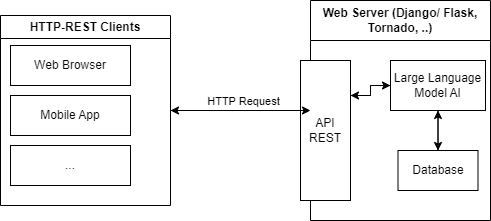
\includegraphics[scale=0.75]{./Figuras/diagBloques.png}
	\caption{Diagrama en bloques del sistema.}
	\label{fig:diagBloques}
\end{figure}
\vspace{25px}

En resumen, la propuesta de valor de este proyecto es la implementación de una serie de servicios REST que serán accedidos por aplicaciones externas,
principalmente Critical Match. Estos servicios permitirán la generación de elementos de ambientación narrativa, basados en el contexto del mundo proporcionado por los usuarios.

Esta iniciativa supone una evolución natural de la App Critical Match.
Actualmente el producto dispone de la funcionalidad de crear mesas y reunir jugadores y esta propuesta añade valor al facilitar a los organizadores de las partidas la creación de contenido atractivo para todos los participantes.

Además, este proyecto podría encajar en otros ámbitos que actualmente están enfocados en el “World Building” al proporcionar a creadores de mundos y escritores herramientas para expandir sus ideas.

Este proyecto a su vez es escalable y permite añadir nuevos servicios con el paso del tiempo.
Esto podría llevar en un futuro a la posibilidad de ofrecer un director de juego automatizado por Inteligencia Artificial que sea de interpretar las reglas y acciones de sus jugadores,
llevando a cabo partidas de rol de manera autónoma.


\section{2. Identificación y análisis de los interesados}
\label{sec:interesados}

\begin{table}[ht]
	%\caption{Identificación de los interesados}
	%\label{tab:interesados}
	\begin{tabularx}{\linewidth}{@{}|l|X|X|l|@{}}
		\hline
		\rowcolor[HTML]{C0C0C0}
		Rol         & Nombre y Apellido & Organización    & Puesto                        \\ \hline
		Cliente     & \clientename      & \empclientename & co-fundador de Critical Match \\ \hline
		Responsable & \authorname       & FIUBA           & Alumno                        \\ \hline
		Director    & \supname          & \pertesupname   & Director Trabajo final        \\ \hline
	\end{tabularx}
\end{table}

De esta lista podemos destacar:
\begin{itemize}
	\item Cliente y usuario final: \clientename.
	      Aporta contexto necesario sobre la App Critical Match y es el interesado de las herramientas que se desarrollarán en el proyecto.
	      Punto de contacto entre el responsable del proyecto y el equipo de Critical Match.
\end{itemize}

\section{3. Propósito del proyecto}
\label{sec:proposito}
El propósito del proyecto es el desarrollo de un servidor web que aloje una Inteligencia Artificial de tipo LLM.
Esta IA será entrenada para la generación de contexto y contenido narrativo.
El servidor podrá recibir peticiones a través del protocolo API REST,
donde se alimentará a la IA con un contexto narrativo.
El servidor responderá las peticiones con la salida aportada por el modelo
dependiendo de la entrada de texto y el tipo de servicio solicitado.


\section{4. Alcance del proyecto}
\label{sec:alcance}

El alcance del proyecto incluye lo siguiente:
\begin{itemize}
	\item Desarrollo de un servidor web.
	\item Entrenamiento de una Inteligencia Artificial de tipo LMM.
	\item Análisis y tratamiento de los datos utilizados para el entrenamiento de la IA.
	\item La integración de un conjunto esencial de servicios REST.
	\item Servicios adicionales, si entran dentro de las horas estimadas del proyecto.
\end{itemize}

El alcance del proyecto no incluye:
\begin{itemize}
	\item Página web.
	\item Securización del servidor web ni de ninguno de sus servicios REST.
	\item Rendimiento de los servicios que garanticen tiempos de respuesta cercanos a tiempo real.
\end{itemize}

En resumen, el proyecto consistirá de un prototipo que aporte funcionalidad en un tiempo de respuesta razonable,
pero es posible que no se ajuste a los requerimientos de un sistema puesto en producción.
Con esto aclarado, la intención siempre será desarrollar el proyecto aportando el mayor rendimiento posible.


\section{5. Supuestos del proyecto}
\label{sec:supuestos}
Para el desarrollo del presente proyecto se supone que:

\begin{itemize}
	\item No se desarrollará la Inteligencia Artificial desde cero, si no que se utilizará una pre-entrenada y de código abierto.
	      Partiendo de esa base, se hara un proceso de \textit{fine-tuning} para especializar el modelo en los servicios de generación de contenido narrativo.
	\item No se dispone de un set de datos por parte del cliente.
	      Se analizarán sets de datos con licencia abierta en la red y se emplearán aquellos que se ajusten al proyecto.
	\item Comunicación fluida con el Equipo de Critical Match para seguimiento del proyecto y aportación de ideas.
	\item El proyecto se realizará con una máquina cuyas especificaciones permitan tanto el desarrollo del código como su ejecución, además del proceso de \textit{fine-tuning} de la Inteligencia artificial.
	\item La disponibilidad para realizar las tareas del proyecto, las cuales se describirán más adelante, será de entre 20 y 30 horas semanales.
\end{itemize}


\section{6. Requerimientos}
\label{sec:requerimientos}
\begin{enumerate}
	\item Requerimientos del servidor:
	      \begin{enumerate}
		      \item El servidor debe alojar y administrar la información relativa al \textit{dataset} y la configuración del modelo LLM.
		      \item El servidor debe contar con los procesos necesarios para entrenar la Inteligencia Artificial.
		      \item Al ser desplegado, el servidor deberá desplegar el módulo LLM y utilizarlo en el procesamiento de peticiones entrantes.
		      \item El servidor debe dar acceso a clientes externos a través del protocolo API REST.
		      \item Los servicios REST deben aceptar entrada de texto en varios formatos: pdf, txt, word o texto plano en el cuerpo de la petición.
		      \item Los servicios REST devolverán la respuesta en formato simple HTML para su cómoda visualización en un navegador.
		      \item El prototipo del servidor debe de tener una disponibilidad del 100\% durante las pruebas y aceptar la carga de trabajo de peticiones individuales.
		            Opcionalmente, sería deseable que maneje el mayor número de peticiones simultáneas posible.
	      \end{enumerate}
	\item Requerimientos del módulo LLM:
	      \begin{enumerate}
		      \item El módulo LLM debe aceptar entrada de texto y generar texto como salida.
		      \item El módulo LLM, si el texto de entrada es legible, debe aportar una respuesta con un detalle y profundidad razonables,
		            además de ser coherente con las instrucciones recibidas.
		      \item El módulo debe disponer de múltiples métodos para los cuales, dada la misma entrada de texto, devolverá información enfocada en un aspecto concreto de la narrativa.
		            Por ejemplo, un método centrado en la generación de personajes, otro en la descripción de localizaciones, un tercero de eventos y así sucesivamente.
		      \item El tiempo de respuesta del módulo LLM debe estar, teniendo en cuenta el \textit{hardware} con el que se dispone, la extensión del texto de entrada y que no se garantiza un rendimiento cercano a tiempo real,
		            en un rango de tiempo razonable para un servicio REST (no más de 5 minutos\textcolor{red}{-desconozco si es un rango de tiempo realista-}).
	      \end{enumerate}
	\item Requerimiento de testing:
	      \begin{enumerate}
		      \item El proyecto contará con test automáticos que probarán el correcto funcionamiento de los módulos no relacionados con el modelo LLM.
		      \item El cliente podrá validar los test automáticos a través de un análisis del código.
		      \item Se validará con el cliente tanto el módulo LLM como el servidor.
	      \end{enumerate}
	\item Requerimientos de documentación:
	      \begin{enumerate}
		      \item Se entregará un documento de administrador que explicará brevemente el sistema, qué comandos de ejecución tiene y los requisitos \textit{hardware} necesarios para su correcto funcionamiento.
		            Además, contará con una descripción de todos los servicios REST disponibles en el servidor y un ejemplo de cómo acceder a ellos.
		            Este documento también recopilará las instrucciones de despliegue con la creación del entorno virtual, instalación de librerías y el entrenamiento del modelo, entre otros.
		      \item Se entregará un documento con un breve análisis de los resultados del módulo LLM que se hayan expuesto al cliente durante las reuniones de seguimiento.
	      \end{enumerate}
	\item Requerimientos legales:
	      \begin{enumerate}
		      \item Cualquier información del cliente que se utilice en el desarrollo del proyecto estará amparada por derechos de privacidad y propiedad intelectual.
		      \item El set de datos utilizado para el entrenamiento del módulo LLM debe tener una licencia libre o que se ajuste a uso académico.
		      \item Todas las librerías de código empleadas en el desarrollo del proyecto deben tener una licencia de código abierto.
	      \end{enumerate}
\end{enumerate}


\section{7. Historias de usuarios (\textit{Product backlog})}
\label{sec:backlog}
A las historias de usuario se les asignará una puntuación (\textit{Story Points}) que seguirá la sucesión de Fibonnaci en un rango de 1 a 13 en función de la dificultad.
A mayor dificultad más tiempo de desarrollo se le dedicará a la historia de usuario y mayores serán los riesgos que acarrea.

A continuación, se describen brevemente los roles:
\begin{itemize}
	\item Administrador: persona o equipo encargado de, sin necesidad de tener conocimiento del código, controlar y monitorizar el estado del sistema en producción.
	\item Desarrollador: persona o equipo con conocimientos de análisis de datos y/o programación encargado de mantener el software.
	\item Usuario: conjunto de personas interesadas en consumir el producto que ofrece el sistema.
\end{itemize}

La lista de historias de usuario es la siguiente:
\begin{itemize}
	\item Como administrador quiero contar con un servidor web y con las herramientas necesarias para su despliegue y detención. (2 puntos)
	\item Como desarrollador deseo tener herramientas que comprueben el buen funcionamiento del código. (5 puntos)
	\item Como desarrollador necesito ser capaz de actualizar el \textit{dataset} y reentrenar la inteligencia artificial. (8 puntos)
	\item Como usuario quiero enviar peticiones API REST al servidor y, aportando un contexto inicial, obtener ambientación narrativa relativa al servicio que he solicitado. (13 puntos)
	\item Como usuario necesito adjuntar archivos de texto en sus formatos habituales (pdf, txt, doc) y que el servicio sea capaz de interpretarlos. (2 puntos)
\end{itemize}


\section{8. Entregables principales del proyecto}
\label{sec:entregables}
\begin{itemize}
	\item Código fuente.
	\item Manual de administrador.
	\item Análisis del \textit{dataset}.
	\item Recopilación de informes de seguimiento del módulo LLM.
	\item Memoria técnica.
\end{itemize}


\section{9. Desglose del trabajo en tareas}
\label{sec:wbs}
\begin{enumerate}
	\item Tareas del servidor (190 h)
	      \begin{enumerate}
		      \item Desarrollo inicial del servidor web y página principal. (20 h)
		      \item Implementación del modelo de datos y ORM (\textit{Object-Relational Mapping}). (40 h)
		      \item Implementación de pruebas automáticas. (40 h)
		      \item Validación de pruebas automáticas. (10 h)
		      \item Implementación del comando para reentrenar el módulo LLM. (20 h)
		      \item Implementación de los servicios API REST del paquete MVP (\textit{Minimum Viable Product} o Producto Viable Mínimo). (20 h)
		      \item Opcional. Implementación de servicios REST adicionales. (40 h)
	      \end{enumerate}
	\item Tareas del módulo LLM (360 h)
	      \begin{enumerate}
		      \item Obtención y análisis inicial del \textit{dataset}. (40 h)
		      \item Desarrollo de software necesario para el tratamiento de los datos (40 h)
		      \item Implementar \textit{pipeline} de procesamiento del \textit{dataset}. (40 h)
		      \item \textit{Fine-tuning} del módulo LLM inicial. (40 h)
		      \item Implementación de los métodos del módulo LLM para el paquete MVP. (40 h)
		      \item Presentación al cliente y análisis inicial de los resultados. (20 h)
		      \item Mejora del \textit{pipeline} de procesamiento del \textit{dataset}. (40 h)
		      \item \textit{Fine-tuning} final del módulo LLM. (40 h)
		      \item Presentación al cliente y análisis final de los resultados. (20 h)
		      \item Opcional. Implementación de métodos del módulo LLM adicionales. (40 h)
	      \end{enumerate}
	\item Tareas de documentación (145 h)
	      \begin{enumerate}
		      \item Plan de proyecto. (20h)
		      \item Presentación del plan de proyecto. (10h)
		      \item Manual de administrador. (10h)
		      \item Documento de análisis del \textit{dataset}. (25 h)
		      \item Recopilación de informes de seguimiento del módulo LLM. (20 h)
		      \item Memoria técnica. (40 h)
		      \item Presentación y defensa del trabajo final. (20 h)
	      \end{enumerate}
\end{enumerate}

Cantidad total de horas: 695 h, de las cuales 80 h son opcionales.
\section{10. Diagrama de Activity On Node}
\label{sec:AoN}
A continuación se presenta en la figura \ref{fig:AoN} el diagrama de \textit{Activity on Node} de las tareas del proyecto.

En la leyenda se indica el color de cada grupo de tareas.
Además, se puede diferenciar el camino crítico en rojo, los caminos semicríticos en amarillo y los caminos opcionales en línea discontinua.
El valor del tiempo de cada tarea está en horas.
\begin{figure}[htpb]
	\centering
	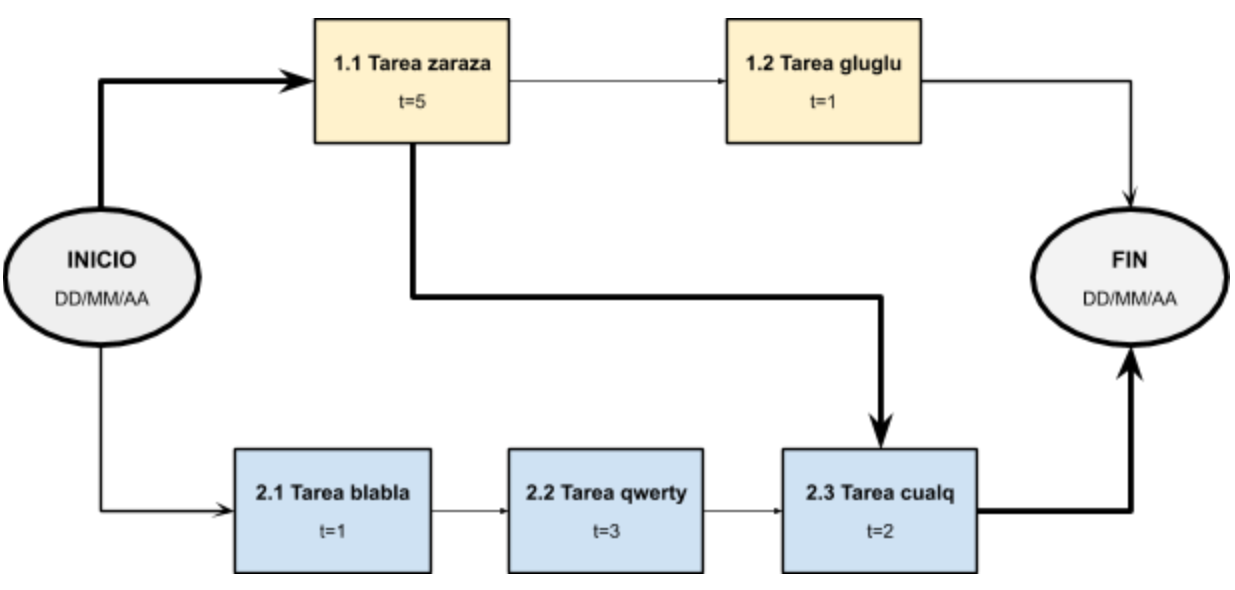
\includegraphics[width=.75\paperwidth]{./Figuras/AoN.png}
	\caption{Diagrama de \textit{Activity on Node}.}
	\label{fig:AoN}
\end{figure}

\section{11. Diagrama de Gantt}
En la figura \ref{fig:diagGantt} se presenta el diagrama de Gantt del proyecto.
Al solo disponer de una persona trabajando en el proyecto, las tareas no pueden paralelizarse y están dispuestas en cascada.
Cada día equivale a 4 horas de trabajo en el proyecto de acuerdo a lo descrito en la sección \ref{sec:supuestos}

Además, las tareas opcionales no aparecen para no desvirtuar el diagrama estimado.
En caso de aplicarse estos objetivos secundarios, se enviará una actualizacion de dicho diagrama a los interesados.

\label{sec:gantt}
\begin{landscape}
	\begin{figure}[htpb]
		\centering
		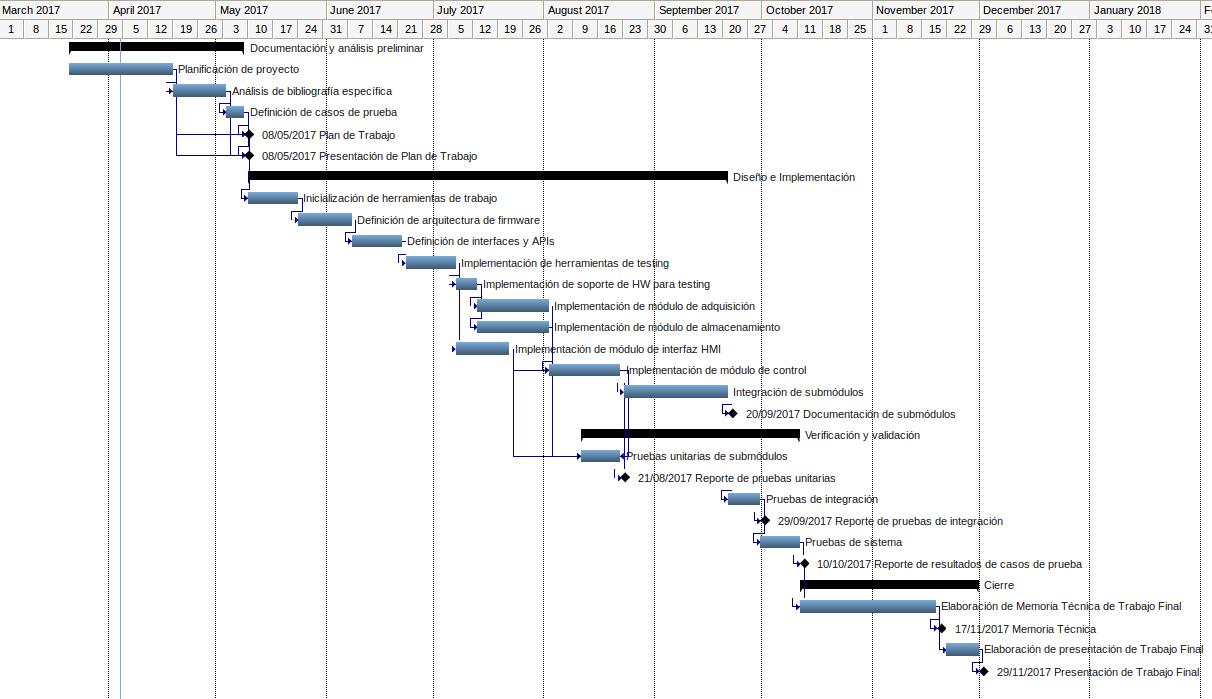
\includegraphics[height=.67\textheight]{./Figuras/Gantt-2.png}
		\caption{Diagrama de Gantt.}
		\label{fig:diagGantt}
	\end{figure}
\end{landscape}
\section{12. Presupuesto detallado del proyecto}
\label{sec:presupuesto}
Para el cómputo del valor de las horas de ingeniería se ha tomado como referencia el salario medio de un ingeniero software en españa en el año 2023, cuyo valor es de \euro18,08 por hora.
Dicho valor se ha convertido a pesos argentinos bajo la tasa representativa del mercado del día 14/11/2023, una equivalencia de 380,96 pesos por euro.
Es decir, el valor del trabajo de ingeniería es de \$6.887,76 por hora.

También se utilizara el valor de conversión de euros a pesos para la estimación del coste del \textit{hardware} de trabajo.

\begin{table}[htpb]
	\centering
	\begin{tabularx}{\linewidth}{@{}|X|c|r|r|@{}}
		\hline
		\rowcolor[HTML]{C0C0C0}
		\multicolumn{4}{|c|}{\cellcolor[HTML]{C0C0C0}COSTOS DIRECTOS}       \\ \hline
		\rowcolor[HTML]{C0C0C0}
		Descripción                                                       &
		\multicolumn{1}{c|}{\cellcolor[HTML]{C0C0C0}Cantidad}             &
		\multicolumn{1}{c|}{\cellcolor[HTML]{C0C0C0}Valor unitario (ARS)} &
		\multicolumn{1}{c|}{\cellcolor[HTML]{C0C0C0}Valor total (ARS)}      \\ \hline
		Horas del Responsable (MVP)                                       &
		\multicolumn{1}{c|}{615}                                          &
		\multicolumn{1}{c|}{6.887,76}                                     &
		\multicolumn{1}{c|}{4.235.972,4}                                    \\ \hline
		Horas del Responsable (Opcional)                                  &
		\multicolumn{1}{c|}{80}                                           &
		\multicolumn{1}{c|}{6.887,76}                                     &
		\multicolumn{1}{c|}{551.020,8}                                      \\ \hline

		\multicolumn{3}{|c|}{SUBTOTAL}                                    &
		\multicolumn{1}{c|}{4.786.993,2}                                    \\ \hline
		\rowcolor[HTML]{C0C0C0}
		\multicolumn{4}{|c|}{\cellcolor[HTML]{C0C0C0}COSTOS INDIRECTOS}     \\ \hline
		\rowcolor[HTML]{C0C0C0}
		Descripción                                                       &
		\multicolumn{1}{c|}{\cellcolor[HTML]{C0C0C0}Cantidad}             &
		\multicolumn{1}{c|}{\cellcolor[HTML]{C0C0C0}Valor unitario (ARS)} &
		\multicolumn{1}{c|}{\cellcolor[HTML]{C0C0C0}Valor total (ARS)}      \\ \hline
		Hardware de trabajo                                               &
		\multicolumn{1}{c|}{1}                                            &
		\multicolumn{1}{c|}{609.536}                                      &
		\multicolumn{1}{c|}{609.536}                                        \\ \hline
		\multicolumn{3}{|c|}{SUBTOTAL}                                    &
		\multicolumn{1}{c|}{609.536}                                        \\ \hline
		\rowcolor[HTML]{C0C0C0}
		\multicolumn{3}{|c|}{TOTAL}                                       &
		\multicolumn{1}{c|}{5.396.529,2}                                    \\ \hline
	\end{tabularx}%
\end{table}

Se aclara de nuevo que \$551.020,8 del coste total se atribuyen a costes opcionales en caso de que se decida añadir funcionalidad adicional.

\section{13. Gestión de riesgos}
\label{sec:riesgos}

\begin{consigna}{red}
	a) Identificación de los riesgos (al menos cinco) y estimación de sus consecuencias:

	Riesgo 1: detallar el riesgo (riesgo es algo que si ocurre altera los planes previstos de forma negativa)
	\begin{itemize}
		\item Severidad (S): mientras más severo, más alto es el número (usar números del 1 al 10).\\
		      Justificar el motivo por el cual se asigna determinado número de severidad (S).
		\item Probabilidad de ocurrencia (O): mientras más probable, más alto es el número (usar del 1 al 10).\\
		      Justificar el motivo por el cual se asigna determinado número de (O).
	\end{itemize}

	Riesgo 2:
	\begin{itemize}
		\item Severidad (S):
		\item Ocurrencia (O):
	\end{itemize}

	Riesgo 3:
	\begin{itemize}
		\item Severidad (S):
		\item Ocurrencia (O):
	\end{itemize}


	b) Tabla de gestión de riesgos:      (El RPN se calcula como RPN=SxO)

	\begin{table}[htpb]
		\centering
		\begin{tabularx}{\linewidth}{@{}|X|c|c|c|c|c|c|@{}}
			\hline
			\rowcolor[HTML]{C0C0C0}
			Riesgo & S & O & RPN & S* & O* & RPN* \\ \hline
			       &   &   &     &    &    &      \\ \hline
			       &   &   &     &    &    &      \\ \hline
			       &   &   &     &    &    &      \\ \hline
			       &   &   &     &    &    &      \\ \hline
			       &   &   &     &    &    &      \\ \hline
		\end{tabularx}%
	\end{table}

	Criterio adoptado:
	Se tomarán medidas de mitigación en los riesgos cuyos números de RPN sean mayores a...

	Nota: los valores marcados con (*) en la tabla corresponden luego de haber aplicado la mitigación.

	c) Plan de mitigación de los riesgos que originalmente excedían el RPN máximo establecido:

	Riesgo 1: plan de mitigación (si por el RPN fuera necesario elaborar un plan de mitigación).
	Nueva asignación de S y O, con su respectiva justificación:
	- Severidad (S): mientras más severo, más alto es el número (usar números del 1 al 10).
	Justificar el motivo por el cual se asigna determinado número de severidad (S).
	- Probabilidad de ocurrencia (O): mientras más probable, más alto es el número (usar del 1 al 10).
	Justificar el motivo por el cual se asigna determinado número de (O).

	Riesgo 2: plan de mitigación (si por el RPN fuera necesario elaborar un plan de mitigación).

	Riesgo 3: plan de mitigación (si por el RPN fuera necesario elaborar un plan de mitigación).

\end{consigna}


\section{14. Gestión de la calidad}
\label{sec:calidad}

\begin{consigna}{red}
	Elija al menos diez requerientos que a su criterio sean los más importantes/críticos/que aportan más valor y para cada uno de ellos indique las acciones de verificación y validación que permitan asegurar su cumplimiento.

	\begin{itemize}
		\item Req \#1: copiar acá el requerimiento.

		      \begin{itemize}
			      \item Verificación para confirmar si se cumplió con lo requerido antes de mostrar el sistema al cliente. Detallar
			      \item Validación con el cliente para confirmar que está de acuerdo en que se cumplió con lo requerido. Detallar
		      \end{itemize}

	\end{itemize}

	Tener en cuenta que en este contexto se pueden mencionar simulaciones, cálculos, revisión de hojas de datos, consulta con expertos, mediciones, etc.  Las acciones de verificación suelen considerar al entregable como ``caja blanca'', es decir se conoce en profundidad su funcionamiento interno.  En cambio, las acciones de validación suelen considerar al entregable como ``caja negra'', es decir, que no se conocen los detalles de su funcionamiento interno.

\end{consigna}

\section{15. Procesos de cierre}
\label{sec:cierre}

\begin{consigna}{red}
	Establecer las pautas de trabajo para realizar una reunión final de evaluación del proyecto, tal que contemple las siguientes actividades:

	\begin{itemize}
		\item Pautas de trabajo que se seguirán para analizar si se respetó el Plan de Proyecto original:
		      - Indicar quién se ocupará de hacer esto y cuál será el procedimiento a aplicar.
		\item Identificación de las técnicas y procedimientos útiles e inútiles que se emplearon, y los problemas que surgieron y cómo se solucionaron:
		      - Indicar quién se ocupará de hacer esto y cuál será el procedimiento para dejar registro.
		\item Indicar quién organizará el acto de agradecimiento a todos los interesados, y en especial al equipo de trabajo y colaboradores:
		      - Indicar esto y quién financiará los gastos correspondientes.
	\end{itemize}

\end{consigna}


\end{document}
